% -*- coding: utf-8 -*-
%-------------------------designed by zcf--------------
\documentclass[UTF8,a4paper,10pt]{ctexart}
\usepackage[left=3.17cm, right=3.17cm, top=2.74cm, bottom=2.74cm]{geometry}
\usepackage{amsmath}
\usepackage{graphicx,subfig}
\usepackage{float}
\usepackage{cite}
\usepackage{caption}
\usepackage{enumerate}
\usepackage{booktabs} %表格
\usepackage{multirow}
\newcommand{\tabincell}[2]{\begin{tabular}{@{}#1@{}}#2\end{tabular}}  %表格强制换行
%-------------------------字体设置--------------
% \usepackage{times} 
\usepackage{ctex}
\setCJKmainfont[ItalicFont=Noto Sans CJK SC Bold, BoldFont=Noto Serif CJK SC Black]{Noto Serif CJK SC}
\newcommand{\yihao}{\fontsize{26pt}{36pt}\selectfont}           % 一号, 1.4 倍行距
\newcommand{\erhao}{\fontsize{22pt}{28pt}\selectfont}          % 二号, 1.25倍行距
\newcommand{\xiaoer}{\fontsize{18pt}{18pt}\selectfont}          % 小二, 单倍行距
\newcommand{\sanhao}{\fontsize{16pt}{24pt}\selectfont}  %三号字
\newcommand{\xiaosan}{\fontsize{15pt}{22pt}\selectfont}        % 小三, 1.5倍行距
\newcommand{\sihao}{\fontsize{14pt}{21pt}\selectfont}            % 四号, 1.5 倍行距
\newcommand{\banxiaosi}{\fontsize{13pt}{19.5pt}\selectfont}    % 半小四, 1.5倍行距
\newcommand{\xiaosi}{\fontsize{12pt}{18pt}\selectfont}            % 小四, 1.5倍行距
\newcommand{\dawuhao}{\fontsize{11pt}{11pt}\selectfont}       % 大五号, 单倍行距
\newcommand{\wuhao}{\fontsize{10.5pt}{15.75pt}\selectfont}    % 五号, 单倍行距
%-------------------------章节名----------------
\usepackage{ctexcap} 
\CTEXsetup[name={,、},number={ \chinese{section}}]{section}
\CTEXsetup[name={(,)},number={\chinese{subsection}}]{subsection}
\CTEXsetup[name={,.},number={\arabic{subsubsection}}]{subsubsection}
%-------------------------页眉页脚--------------
\usepackage{fancyhdr}
\pagestyle{fancy}
\lhead{\kaishu \leftmark}
% \chead{}
\rhead{\kaishu 计算机网络第一次实验}%加粗\bfseries 
\lfoot{}
\cfoot{\thepage}
\rfoot{}
\renewcommand{\headrulewidth}{0.1pt}  
\renewcommand{\footrulewidth}{0pt}%去掉横线
\newcommand{\HRule}{\rule{\linewidth}{0.5mm}}%标题横线
\newcommand{\HRulegrossa}{\rule{\linewidth}{1.2mm}}
%-----------------------伪代码------------------
\usepackage{algorithm}  
\usepackage{algorithmicx}  
\usepackage{algpseudocode}  
\floatname{algorithm}{Algorithm}  
\renewcommand{\algorithmicrequire}{\textbf{Input:}}  
\renewcommand{\algorithmicensure}{\textbf{Output:}} 
\usepackage{lipsum}  
\makeatletter
\newenvironment{breakablealgorithm}
  {% \begin{breakablealgorithm}
  \begin{center}
     \refstepcounter{algorithm}% New algorithm
     \hrule height.8pt depth0pt \kern2pt% \@fs@pre for \@fs@ruled
     \renewcommand{\caption}[2][\relax]{% Make a new \caption
      {\raggedright\textbf{\ALG@name~\thealgorithm} ##2\par}%
      \ifx\relax##1\relax % #1 is \relax
         \addcontentsline{loa}{algorithm}{\protect\numberline{\thealgorithm}##2}%
      \else % #1 is not \relax
         \addcontentsline{loa}{algorithm}{\protect\numberline{\thealgorithm}##1}%
      \fi
      \kern2pt\hrule\kern2pt
     }
  }{% \end{breakablealgorithm}
     \kern2pt\hrule\relax% \@fs@post for \@fs@ruled
  \end{center}
  }
\makeatother
%------------------------代码-------------------
\usepackage{xcolor} 
\usepackage{listings} 
\lstset{ 
breaklines,%自动换行
basicstyle=\small,
escapeinside=``,
keywordstyle=\color{ blue!70} \bfseries,
commentstyle=\color{red!50!green!50!blue!50},% 
stringstyle=\ttfamily,% 
extendedchars=false,% 
linewidth=\textwidth,% 
numbers=left,% 
numberstyle=\tiny \color{blue!50},% 
frame=trbl% 
rulesepcolor= \color{ red!20!green!20!blue!20} 
}
%------------超链接----------
\usepackage[colorlinks,linkcolor=black,anchorcolor=blue]{hyperref}
%------------------------TODO-------------------
\usepackage{enumitem,amssymb}
\newlist{todolist}{itemize}{2}
\setlist[todolist]{label=$\square$}
% for check symbol 
\usepackage{pifont}
\newcommand{\cmark}{\ding{51}}%
\newcommand{\xmark}{\ding{55}}%
\newcommand{\done}{\rlap{$\square$}{\raisebox{2pt}{\large\hspace{1pt}\cmark}}\hspace{-2.5pt}}
\newcommand{\wontfix}{\rlap{$\square$}{\large\hspace{1pt}\xmark}}
%------------------------水印-------------------
\usepackage{tikz}
\usepackage{xcolor}
\usepackage{eso-pic}

\newcommand{\watermark}[3]{\AddToShipoutPictureBG{
\parbox[b][\paperheight]{\paperwidth}{
\vfill%
\centering%
\tikz[remember picture, overlay]%
  \node [rotate = #1, scale = #2] at (current page.center)%
    {\textcolor{gray!80!cyan!30!magenta!30}{#3}};
\vfill}}}



%———————————————————————————————————————————正文———————————————————————————————————————————————
%----------------------------------------------
\begin{document}
\begin{titlepage}
    \begin{center}
    
\includegraphics[width=0.8\textwidth]{NKU.png}\\[1cm]    
    \textsc{\Huge \kaishu{\textbf{南\ \ \ \ \ \ 开\ \ \ \ \ \ 大\ \ \ \ \ \ 学}} }\\[0.9cm]
    \textsc{\huge \kaishu{\textbf{网\ \ 络\ \ 空\ \ 间\ \ 安\ \ 全\ \ 学\ \ 院}}}\\[0.5cm]
    \textsc{\Large \textbf{计算机网络实验3-1}}\\[0.8cm]
    \HRule \\[0.9cm]
    { \LARGE \bfseries 基于UDP服务设计可靠传输协议并编程实现}\\[0.4cm]
    \HRule \\[2.0cm]
    \centering
    \textsc{\LARGE \kaishu{\ \ 马世骐 \ \ 6016252}}\\[0.5cm]
    \textsc{\LARGE \kaishu{年级\ :\ 2020级}}\\[0.5cm]
    \textsc{\LARGE \kaishu{专业\ :\ 经济伯苓班}}\\[0.5cm]
    \textsc{\LARGE \kaishu{指导教师\ :\ 张建忠、徐敬东}}\\[0.5cm]
    \vfill
    {\Large \today}
    \end{center}
\end{titlepage}
%-------------摘------要--------------
\newpage
\thispagestyle{empty}
%----------------------------------------------------------------
\tableofcontents
%----------------------------------------------------------------
\newpage
\watermark{60}{10}{NKU}
\setcounter{page}{1}
%----------------------------------------------------------------
\section{实验基本描述}
%——————————————————————————————————————
利用数据报套接字在用户空间实现面向连接的可靠数据传输,功能包括如下内容:
\begin{enumerate}
  \item 建立连接
  \item 差错检测
  \item 确认重传
  \item 停等机制
  \item 断开连接
\end{enumerate}

%----------------------------------------------------------------
\section{实验具体工作}
%——————————————————————————————————————
\subsection{协议设计}
\subsubsection{报文格式}
\begin{figure}[H]
    \centering
    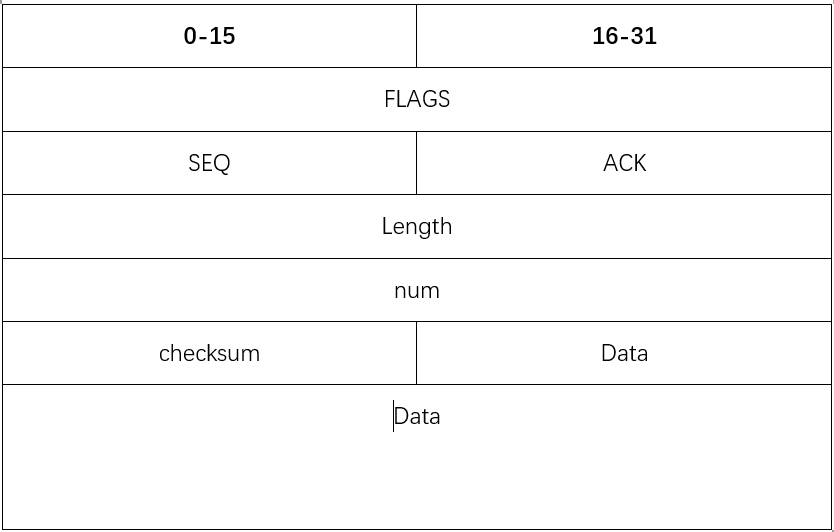
\includegraphics[scale=0.6]{计网1.png}
    \label{fig:1}
\end{figure}
\begin{lstlisting}[title=报文格式,frame=trbl,language={C++}]
struct message
{
#pragma pack(1)
    u_long flag{};
    u_short seq{};//序列号
    u_short ack{};//确认号
    u_long len{};//数据部分长度
    u_long num{}; //发送的消息包含几个包
    u_short checksum{};//校验和
    char data[1024]{};//数据长度
#pragma pack()
}
\end{lstlisting}
flags为我们所设计的伪首部,其中包含了SYN、FIN、START、END位,分别表示包的基本信息,还有一个EXIST位,表示包不为空(由于我们使用非阻塞模式,需要有此设置)。这五位,分别由flags的第一位、第二位、第四位、第八位、第十六位表示,其他位由0补齐。\par
我们的DATA为所传输的图片或文字的部分,其长度设置为1024。
\subsubsection{状态转换图}
采用类似于rdt3.0的状态转换机制,大致如下所示:
\begin{figure}[H]
    \centering
    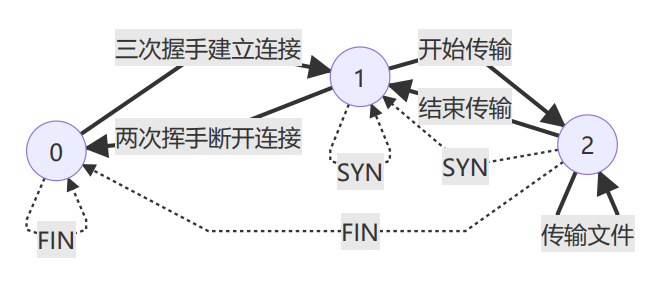
\includegraphics[scale=0.8]{计网3.png}
    \label{fig:3}
\end{figure}
本程序的文件传输流程如下,后文将具体介绍:
\begin{figure}[H]
    \centering
    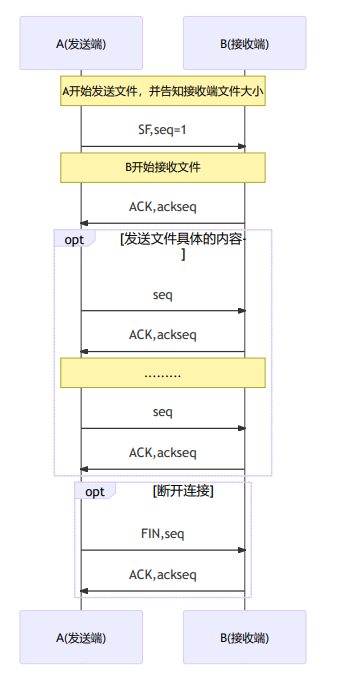
\includegraphics[scale=1.0]{计网4.png}
    \caption{无异常情况下的发送流程}
    \label{fig:4}
\end{figure}

\begin{figure}[H]
    \centering
    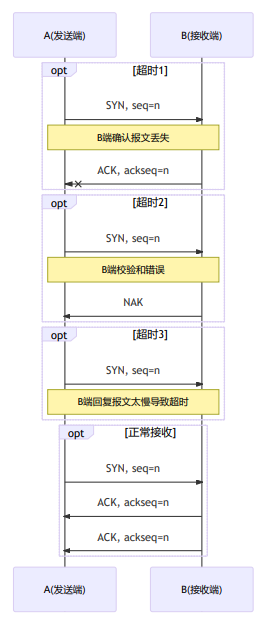
\includegraphics[scale=1.0]{计网5.png}
    \caption{异常情况下的发送流程}
    \label{fig:5}
\end{figure}
\subsubsection{建立连接}
建立连接的过程,仿照了三次握手的过程,客户端发送带有标识SYN的消息x,接收到对方对消息x的确认消息ACK。由客户端发出第一次握手的请求,然后服务器发回第二次握手,唯一的区别是我这里客户端发出的第三次握手并不会真的被服务器收到,原因很简单,因为我们是单向传输的。
下面是大致的流程图:
\begin{figure}[H]
    \centering
    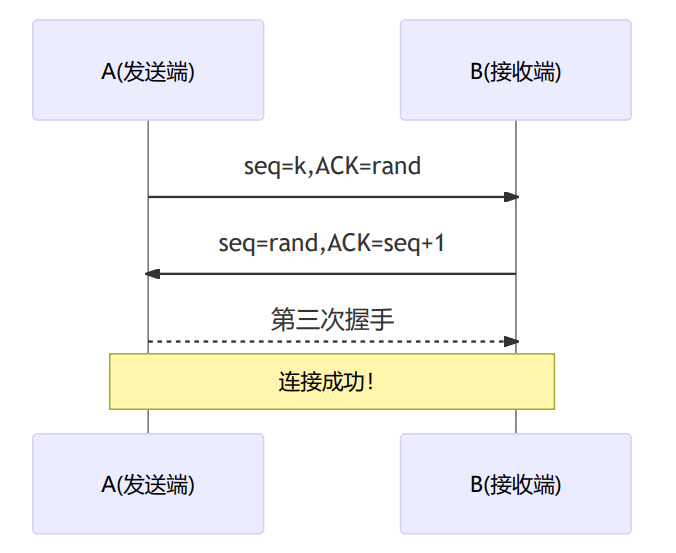
\includegraphics[scale=0.6]{计网2.png}
    \label{fig:2}
\end{figure}
具体代码实现如下所示:
\begin{lstlisting}[title=客户端,frame=trbl,language={C++}]
int beginconnect()
{
    SetColor(0,12);
    cout << "开始连接!发送第一次握手!" << endl;
    message recvMsg, sendMsg;
    sendMsg.setSYN();
    sendMsg.seq = 88;
    sendmessage(sendMsg);
    int start = clock();
    int end;
    while (true)
    {
        recvMsg = recvmessage();
        if (!recvMsg.isEXT())
        {
            end = clock();
            if (end - start > 2000) {
                SetColor(0,12);
                cout << "连接超时,请确认网络通畅和服务端启动无误后再运行本程序!" << endl;
                break;
            }
            continue;
        }
        if (recvMsg.isACK() && recvMsg.isSYN()&& recvMsg.ack == sendMsg.seq + 1) {
            SetColor(14,0);
            cout << "收到第二次握手!" << endl;
            break;
        }
    }
    sendMsg.setACK();
    sendMsg.seq = 89;
    sendMsg.ack = recvMsg.seq + 1;
    SetColor(14,0);
    cout << "发送第三次握手的数据包" << endl;
    sendmessage(sendMsg);
    return 0;
}
\end{lstlisting}

\begin{lstlisting}[title=服务器,frame=trbl,language={C++}]
int WaitConnect()
{
    SetColor(14,0);
    cout << "服务器等待连接" << endl;
    message recvMsg, sendMsg;
    while (true)
    {
        recvMsg = recvmessage();
        if (recvMsg.isSYN())
        {
            SetColor(14,0);
            cout << "收到第一次握手成功!" << endl;
            break;
        }
    }
    sendMsg.setSYN();
    sendMsg.setACK();
    sendMsg.ack = recvMsg.seq + 1;   // 将要发送确认包的ack设为收到包的seq+1
    sendMsg.setSYN();
    SetColor(14,0);
    cout << "发送第二次握手信息!" << endl;
    sendmessage(sendMsg);
    SetColor(14,0);
    cout << "接收到确认连接,连接成功" << endl;
    int iMode = 0; //1:非阻塞,0:阻塞
    ioctlsocket(Server, FIONBIO, (u_long FAR*) & iMode);//非阻塞设置
    return 0;
}
\end{lstlisting}
\subsubsection{断开连接}
断开连接采用的是两次挥手,由客户端开始发出第一次挥手,服务器收到挥手后返回第二次挥手,然后双方程序结束运行。

具体代码实现如下所示:
\begin{lstlisting}[title=客户端,frame=trbl,language={C++}]
int closeconnect() {  // 断开连接
    message recvMsg, sendMsg;
    sendMsg.setFIN();
    sendMsg.seq = 65534;//此处是u_short的表示范围的最大值-1,而我们收到的将会再加一,那么已经到了u_short的最大值了,就自然结束了。
    sendmessage(sendMsg);
    cout << "发送出去第一次挥手!" << endl;
    int count = 0;
    while (true) {
        Sleep(100);
        if (count >= 50) {
            SetColor(0,12);
            cout << "等待时间太长,退出连接" << endl;
            return closeconnect();
        }
        recvMsg = recvmessage();
        if (!recvMsg.isEXT()) {
            continue;
        }
        if (recvMsg.isACK() && recvMsg.ack == sendMsg.seq + 1) {
            break;
        }
        count++;
    }
    SetColor(0,12);
    cout << "接收到确认连接,断开连接成功" << endl << endl;
    return 0;
}
\end{lstlisting}
客户端此处的第一次挥手有一个小的设计是把seq设置为u\_short的表示范围的最大值-1,而我们收到的将会再加一,那么已经到了u\_short的最大值了,就自然结束了。
\begin{lstlisting}[title=服务器,frame=trbl,language={C++}]
int closeconnect(message msg){
    message sendMsg;
    sendMsg.setACK();
    sendMsg.ack = msg.seq + 1;
    sendmessage(sendMsg);
    SetColor(14,0);
    cout<<"已经收到客户端发过来的挥手请求,并且发送了第二次挥手,服务器将结束运行!再见!"<<endl;
    return 0;
}
\end{lstlisting}
\subsubsection{差错检测}
主要是校验和计算的函数,这个函数修改自老师课上所给出的方法,也就是说,如果校验和为0的话,我们的包就是正确的。具体代码如下:
\begin{lstlisting}[title=校验和计算,frame=trbl,language={C++}]
void setchecksum(){
    int sum = 0;
    u_char* temp = (u_char*)this;
    for (int i = 0; i < 8; i++)
    {
        sum += (temp[i<<1] << 8) + temp[i<<1|1];
        while (sum > 0xffff)
        {
            int t = sum >> 16;  
            sum += t;
        }
    }
    checksum = ~(u_short)sum;  
}
\end{lstlisting}

\subsubsection{确认重传}
前面在连接建立部分已经简要进行介绍,当client端无法在规定时间内接收到相应消息的ACK时,重传消息。那么主要涉及以下几种情况:
\begin{enumerate}
  \item server端检测校验和出错,不发送ACK
  \item server端发送的ACK丢包
  \item server端发送的ACK未在超时时限内收到
\end{enumerate}
\textbf{首先,我把接收的函数封装了,如果遇到上述三种情况(写在条件跳转语句的判定条件之中),我的接收函数并不会返回一个报文,而是刷新message,把他们都置为0,然后重新接收。因此,可以等待至超时。}接收函数如下所示:
\begin{lstlisting}[title=接收函数,frame=trbl,language={C++}]
message recvmessage()
{
    message msg;
    if (recvfrom(Server, (char*)&msg, BUFFER, 0, (SOCKADDR*)&clientaddr, &len) ==-1 || !msg.isEXT() || msg.corrupt()) {
        return message();
    }
    return msg;
}
\end{lstlisting}
这其中的判断主要由以下封装的函数来实现:
\begin{lstlisting}[title=检测,frame=trbl,language={C++}]
bool corrupt(){
    // 包是否损坏
    int sum = 0;
    u_char* temp = (u_char*)this;
    for (int i = 0; i < 8; i++)
    {
        sum += (temp[i<<1] << 8) + temp[i<<1|1];
        while (sum > 0xffff)
        {//溢出
            int t = sum >> 16;//计算方法与设置校验和相同
            sum += t;
        }
    }
    //把计算出来的校验和和报文中该字段的值相加,如果等于0xffff,则校验成功
    if (checksum + (u_short)sum == 65535)
        return false;
    return true;
}
\end{lstlisting}
\textbf{因为我们的设计类似于rdt3.0的设计,此处采用超时重传机制。使用clock()函数进行计时,从发送消息之后就开始计时,一旦时间超过某个限度后仍然没有收到服务器发来的对应的ack,就会重新发送消息。这里注意,我设置了最大的重发次数,此处设为10次,即一旦重发10次仍然没有成功,客户端就不会再重新发送了,因此不会陷入死循环之中。此处设置的意义是,一旦网络不通或服务器关闭,那么不会做无用的尝试。}具体代码如下所示:
\begin{lstlisting}[title=超时重传,frame=trbl,language={C++}]
int waitSend(message sendMsg, int seq)
{
    message recvMsg;
    sendMsg.seq = seq;
    sendmessage(sendMsg);
    int iMode = 1; //1:非阻塞,0:阻塞
    ioctlsocket(Client, FIONBIO, (u_long FAR*) & iMode);//非阻塞设置
    int count = 0;
    clock_t start = clock();
    clock_t end;
    while (1) {
        end = clock();
        if (end - start > 50) {
            SetColor(0,12);
            cout << "应答超时,重新发送数据包" << endl;
            sendmessage(sendMsg);
            count++;
            SetColor(0,12);
            cout<<"尝试重新发送第"<<count<<"次,最多10次"<<endl;
            if(count>=10){
                SetColor(0,12);
                cout << "重发失败,请确认网络通畅以及服务端启动后,重新启动客户端并重新发送文件!再见!" << endl;
                break;
            }
            start = clock();
        }
        recvMsg = recvmessage();
        if (!recvMsg.isEXT()) {
            continue;
        }
        if (recvMsg.isACK() && recvMsg.ack == seq) {
            SetColor(14,0);
            cout << "收到服务器发来的ack正确的确认数据包!" << endl;
            cout << endl;
            return 1;
        }
    }
    return 0;
}
\end{lstlisting}

\subsubsection{停等机制}
该机制下client端每发送一条消息,都需要等待接收到对方返回的ACK才能发送下一条,client端代码与确认重传部分相同,这里对server端代码进行解释,即收到client端的消息且检测校验和正确后,向对方发送相应消息的ACK,代码实现如下所示:
\begin{lstlisting}[title=停等机制,frame=trbl,language={C++}]
if (recvMsg.seq == seq) {
    sendMsg.setACK();
    sendMsg.ack = recvMsg.seq;
    SetColor(14,0);
    cout << "收到seq为" << recvMsg.seq << "的数据包" << endl;
    SetColor(14,0);
    cout << "发送确认收到的数据包(对应的ack)" << endl;
    sendmessage(sendMsg);
    cout << endl;
    out.write(recvMsg.data, recvMsg.len);
    break;
}
\end{lstlisting}
同时,加入了超时检测机制:
\begin{lstlisting}[title=超时的检测,frame=trbl,language={C++}]
end = clock();
if (end - start > 2000) {
    SetColor(14,0);
    cout << "传输超时失败" << endl;
    cout << "请确认网络通畅后重新进行文件接收工作!谢谢!" << endl;
    int iMode = 0; //1:非阻塞,0:阻塞
    ioctlsocket(Server, FIONBIO, (u_long FAR*) & iMode);//非阻塞设置
    return getFileName();
}
\end{lstlisting}
\subsubsection{文件发送}
首先我们需要打开文件,这一步我们统一以二进制的形式打开,这是因为有图片的存在,具体代码如下所示:
\begin{lstlisting}[title=打开文件,frame=trbl,language={C++}]
int openFile() {
    SetColor(0,10);
    cout << "请输入要发送的文件名:";
    memset(filepath, 0, 20);
    string temp;
    cin >> temp;
    if (temp == "FINISH") {
        return closeconnect();
    } else {
        if(temp=="1.jpg"||temp=="2.jpg"||temp=="3.jpg"||temp=="helloworld.txt"){
        strcpy(filepath, temp.c_str());
        in.open(filepath, ifstream::in | ios::binary);// 以二进制方式打开文件
        in.seekg(0, std::ios_base::end);  // 将文件流指针定位到流的末尾
        filelen = in.tellg();
        messagenum = filelen / 1024 + 1;
        SetColor(0,6);
        cout << "文件大小为" << filelen << "Bytes,总共有" << messagenum << "个数据包" << endl;
        in.seekg(0, std::ios_base::beg);  // 将文件流指针定位到流的开始
        return 1;
    }
        else{
            SetColor(0,12);
            cout<<"文件不存在,请重新输入您要传输的文件名!"<<endl;
            return openFile();
        }
    }
}
\end{lstlisting}
\begin{lstlisting}[title=客户端发送文件,frame=trbl,language={C++}]
int sendmessages() {
    SetColor(0,6);
    cout << "开始发送文件内容!" << endl;
    message msg;
    int seq = 1;
    while (filelen) {
        if (filelen > 1024)
        {
            in.read(msg.data, 1024);
            msg.len = 1024;
            filelen -= 1024;
        }
        else
        {
            in.read(msg.data, filelen);
            msg.len = filelen;
            msg.setEND();
            filelen = 0;
        }
        SetColor(14,0);
        cout << "发送seq为" << seq << "的数据包" << endl;
        if (waitSend(msg, seq) == 0) {
            SetColor(0,12);
            cout << "发送seq为" << seq << "的数据包失败!!!" << endl << endl;
            return 0;
        }
        seq++;
    }
    SetColor(0,6);
    cout << "成功发送文件!" << endl;
    timeend = clock();
    double endtime = (double)(timeend - timestart) / CLOCKS_PER_SEC;
    SetColor(0,6);
    in.close();
    in.clear();
    return sendFirstName();  // 准备发送下一个文件
}
\end{lstlisting}

\subsubsection{文件接收}
\begin{lstlisting}[title=服务器接收文件,frame=trbl,language={C++}]
int recvmessages() {
    cout << "开始接收文件内容!" << endl;
    message recvMsg, sendMsg;
    int seq = 1;
    int iMode = 1; //1:非阻塞,0:阻塞
    ioctlsocket(Server, FIONBIO, (u_long FAR*) & iMode);//非阻塞设置
    for (int i = 0; i < messagenum; i++) {
        int start = clock();
        int end;
        while (1) {
            end = clock();
            if (end - start > 2000) {
                SetColor(14,0);
                cout << "传输超时失败" << endl;
                cout << "请确认网络通畅后重新进行文件接收工作!谢谢!" << endl;
                int iMode = 0; //1:非阻塞,0:阻塞
                ioctlsocket(Server, FIONBIO, (u_long FAR*) & iMode);//非阻塞设置
                return getFileName();
            }
            recvMsg = recvmessage();
            if (!recvMsg.isEXT()) {
                continue;
            }
            if (recvMsg.seq == seq) {
                sendMsg.setACK();
                sendMsg.ack = recvMsg.seq;
                SetColor(14,0);
                cout << "收到seq为" << recvMsg.seq << "的数据包" << endl;
                SetColor(14,0);
                cout << "发送确认收到的数据包(对应的ack)" << endl;
                sendmessage(sendMsg);
                cout << endl;
                out.write(recvMsg.data, recvMsg.len);
                break;
            }
        }
        if (recvMsg.isEND()) {
            SetColor(14,0);
            cout << "接收文件成功!!" << endl << endl;
            out.close();
            out.clear();
            int iMode = 0; //1:非阻塞,0:阻塞
            ioctlsocket(Server, FIONBIO, (u_long FAR*) & iMode);//非阻塞设置
            return getFileName();
        }
        seq++;
    }
}
\end{lstlisting}
\subsubsection{丢包设计}
由于所提供的router.exe不能使用,因此我自行设置了一个丢包的函数,原理是设置随机数,然后用随机数mod100,以此设计丢包率,代码如下所示:
\begin{lstlisting}[title=丢包函数,frame=trbl,language={C++}]
int judgeRand(){
    int s=rand()%100;
    if(s<5){return 0;}
    else{return 1;}
}
\end{lstlisting}
\begin{lstlisting}[title=发送函数,frame=trbl,language={C++}]
void sendmessage(message msg) {
    msg.setEXT();
    msg.setchecksum();
    if(judgeRand()==1){
    if (sendto(Client, (char*)&msg, BUFFER, 0, (SOCKADDR*)&serveraddr, sizeof(SOCKADDR)) == (SOCKET_ERROR)) {
        SetColor(0,12);
        cout << "发送错误了!!" << endl;
    }}
}
\end{lstlisting}
\subsection{结果展示}
首先是建立连接的过程:
\begin{figure}[H]
    \centering
    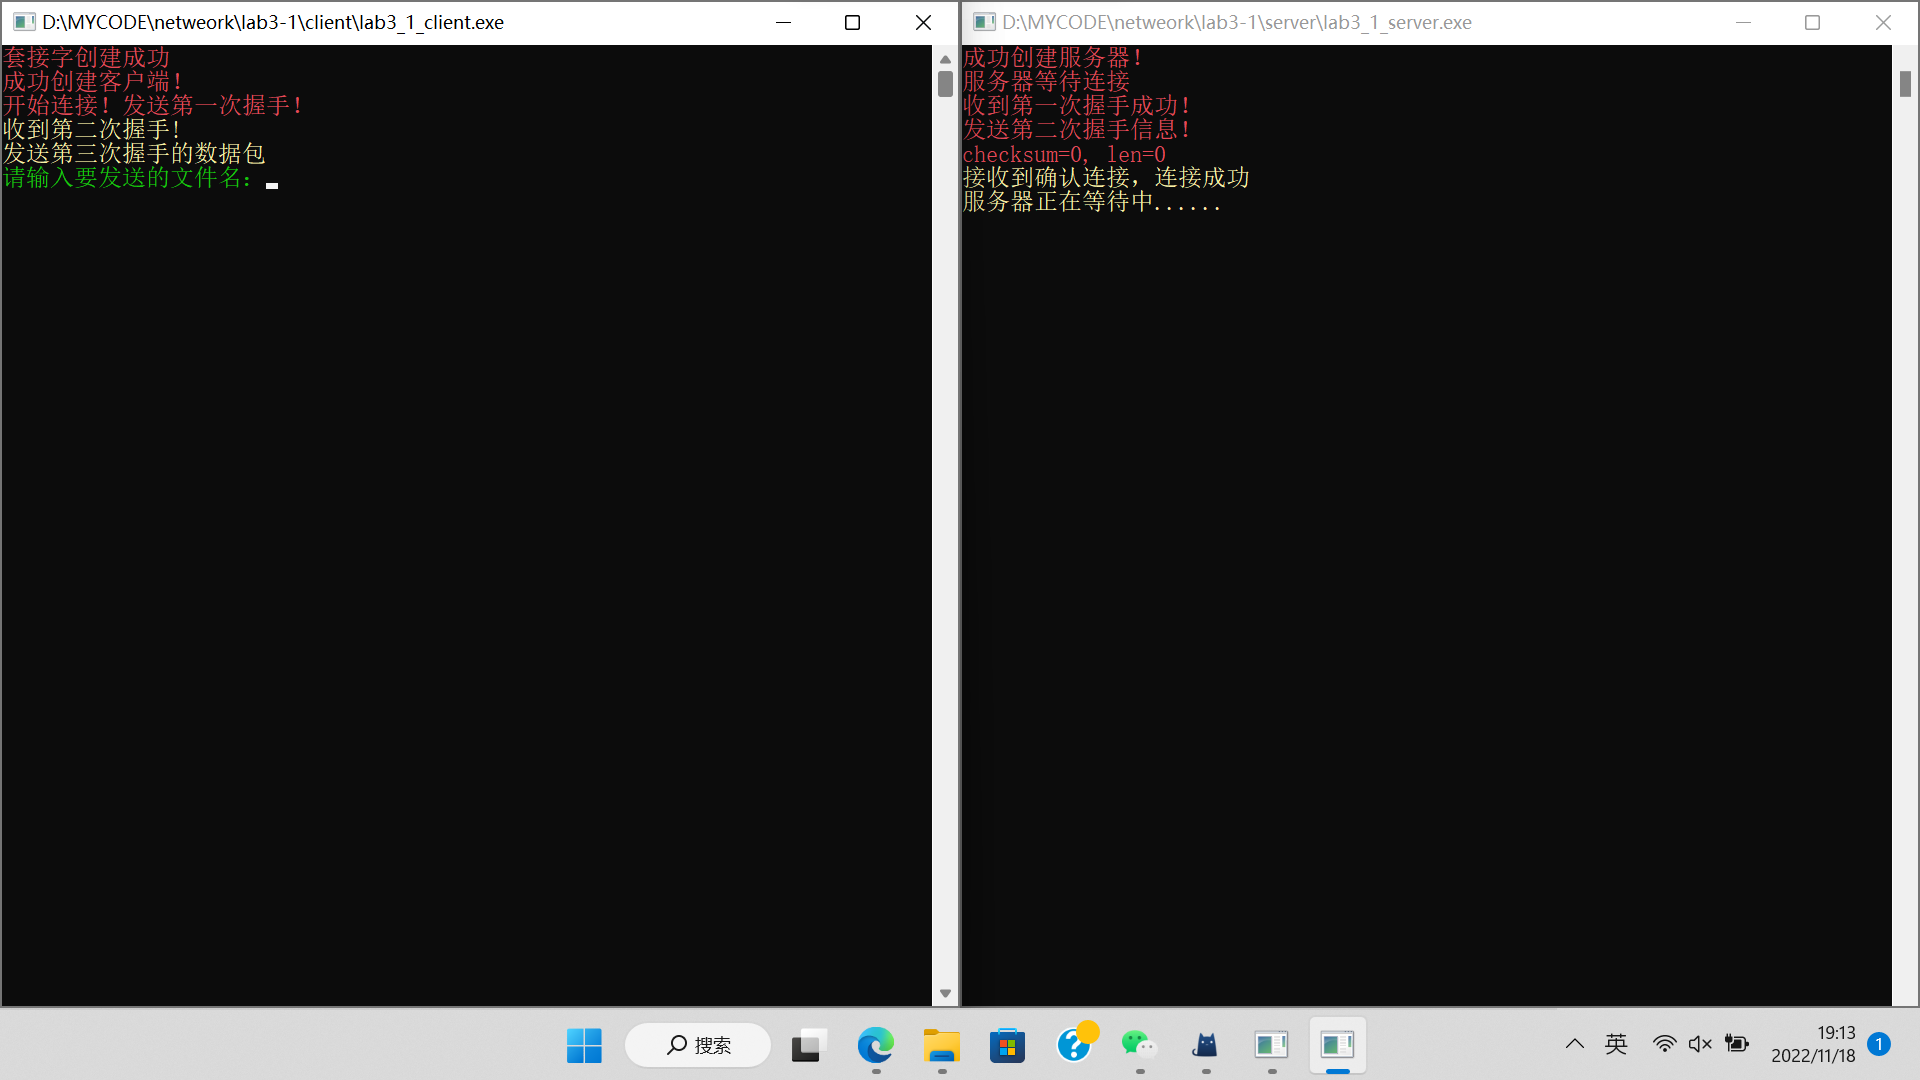
\includegraphics[scale=0.4]{计网6.png}
    \label{fig:6}
\end{figure}
接下来是依次发送文件的过程:
\begin{figure}[H]
    \centering
    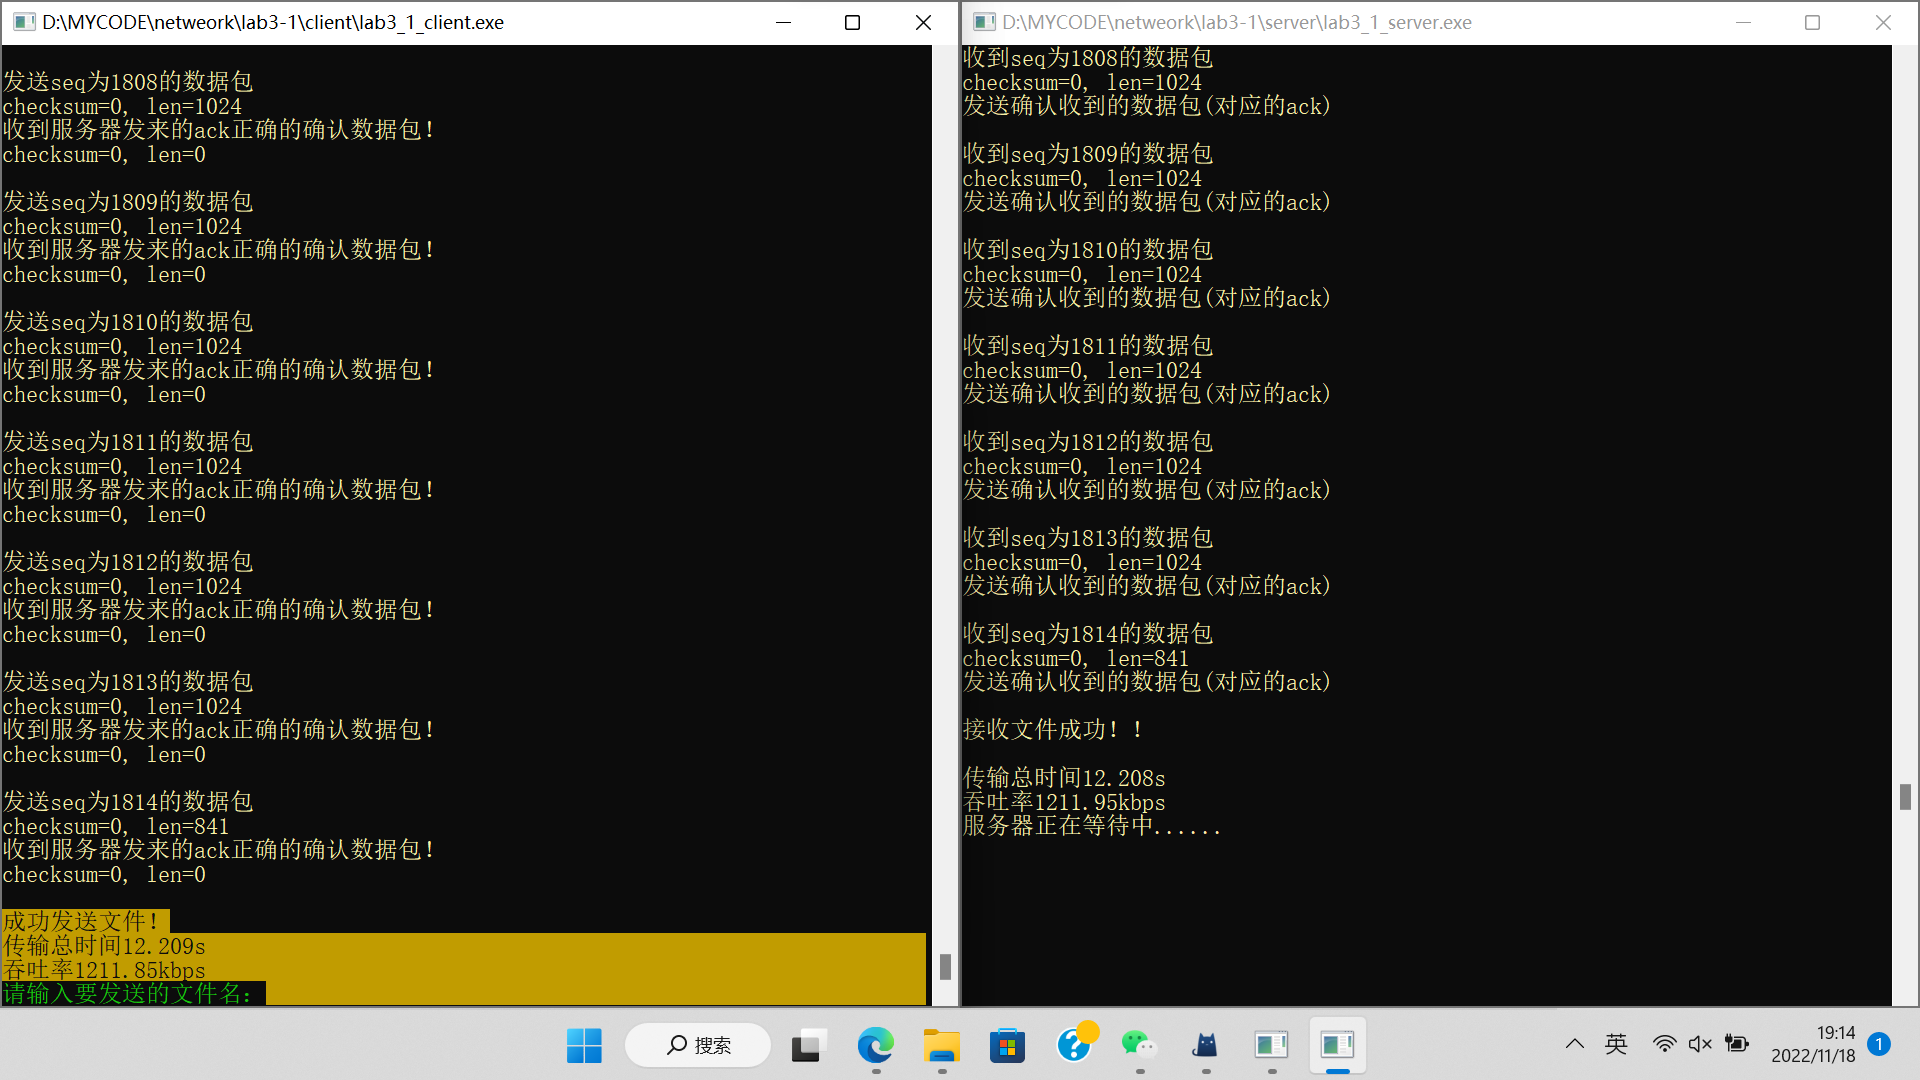
\includegraphics[scale=0.4]{计网7.png}
    \label{fig:7}
\end{figure}
可以看到文件发送成功。此处的日志展示了最后一个包的长度是841而不是我设置的定长1024,说明是成功的。

接下来测试一下重传,我们在发送的过程中,选择关掉服务器程序,展示一下重传机制。这里会看到,客户端会尝试重新发送报文,但是发送十次仍然没有成功后,就选择停止发送了。这是我设置好的阈值。
\begin{figure}[H]
    \centering
    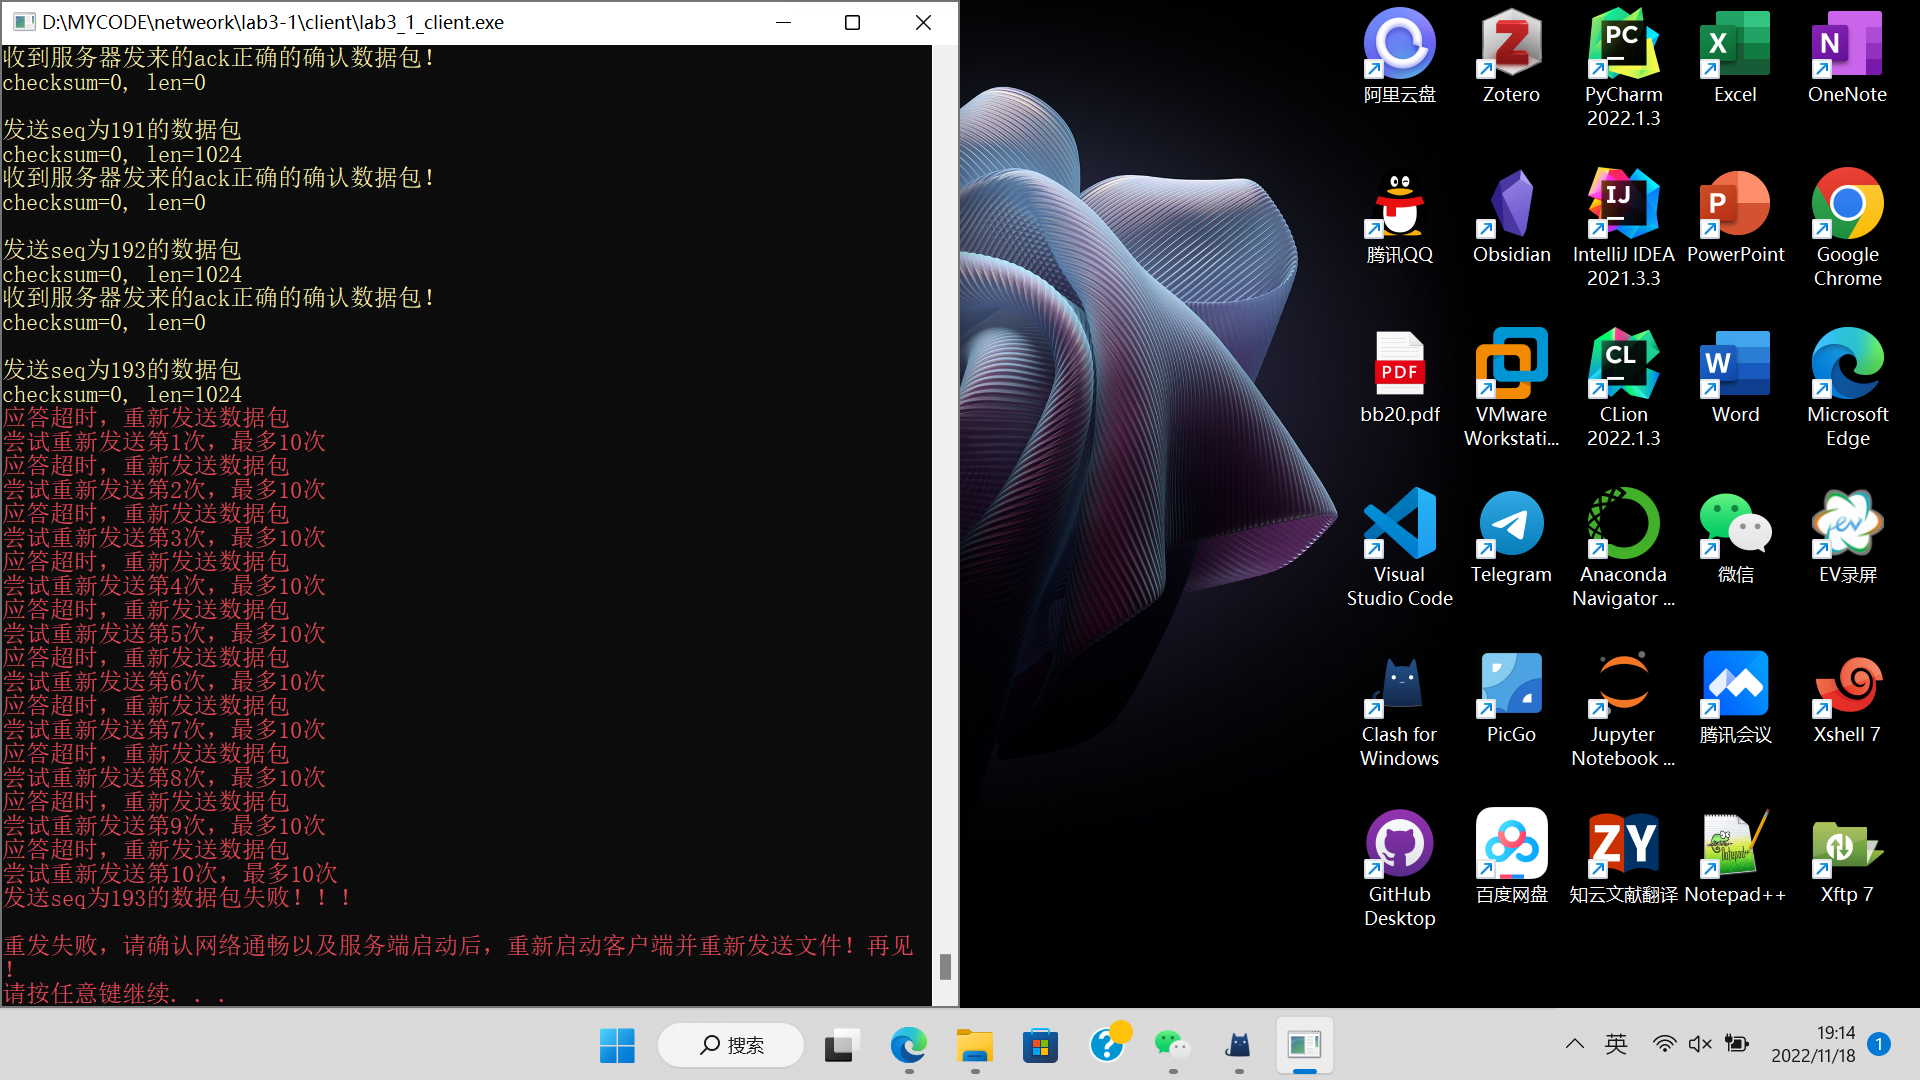
\includegraphics[scale=0.4]{计网8.png}
    \label{fig:8}
\end{figure}
最后断开连接:
\begin{figure}[H]
    \centering
    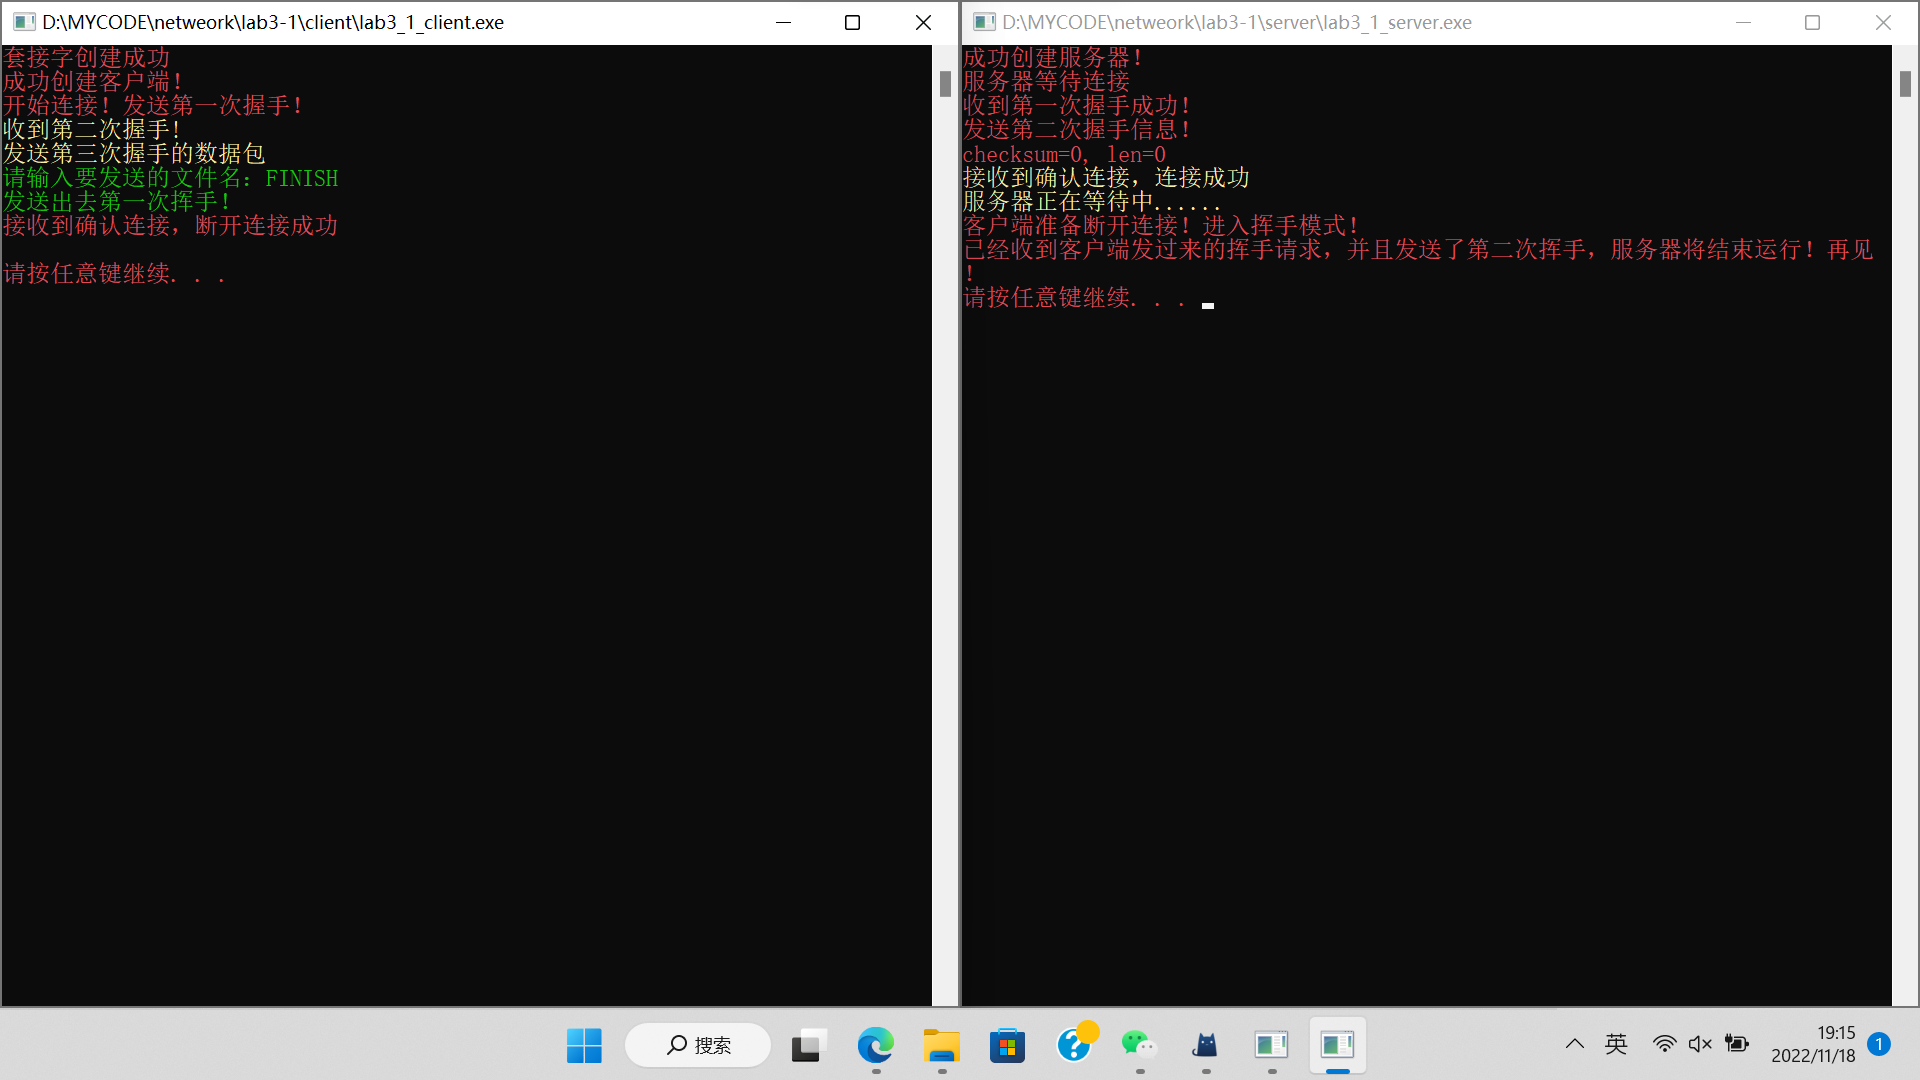
\includegraphics[scale=0.4]{计网9.png}
    \label{fig:9}
\end{figure}
\section{总结与一些问题}
本次实验我基于UDP实现了可靠文件传输,学到了很多。我个人还进行了一些更多思考,本次实验由于是单向的传输,因此协议并不需要非常复杂,比如在握手挥手阶段,这一部分一开始想复杂了。最后,目前还存在一些小的问题是不能由多个IP地址之间进行传输,只能使用127.0.0.1这个回环地址,后续会做进一步优化。
\end{document}